\section{Implementation}
This section gives you additional insight on part of the implementation and discusses challenges and problems encountered. Also gives information on the approaches to solve this issues.

\subsection{Displaying a Map inside Xamarin Forms}
One of the first things that was implemented in the \gls{app}, after getting the basic structure of the \gls{app}, was showing a map. The first implementation was really simple and just showed a map, like the default map \gls{app} on a phone. Afterwards additional functionality was added.

Displaying a map in \gls{XamarinForms} normally is really simple, as you can see on the Xamarin Forms Maps \cite{xamMaps} site, using the \gls{XamarinForms} map component is really simple. Just add a \gls{nuget} package to the project and then display a map with a few lines of code. This is fine if you don't need to extend it, but in our case we wanted to add additional functionality to it.

After determining that something more powerful was needed, different solutions to display the map were considered. Exiting solutions like
OsmSharp \cite{osmsharp}, which provided a good looking map based on open street map, were considered. But they were focused on routing and didn't offer any of the features our \gls{app} needed like adding custom \glspl{overlay} to a map.
Also there are different solutions available that offer extensive server side rendering of maps containing your own data. A popular solution is Mapbox \cite{mapbox}, but using a server backend for the \gls{app} was out of scope for the project so a solution was chosen that would work on the device.

The only usable way we found was to implement our own custom map \gls{renderer} on each platform. This \gls{renderer} is overriding he default map \gls{renderer} on each platform and then adds the custom functionality on top of it. This approach also meant that each feature related to the map needed to be implemented two times. Once for android and once for iOS, which mean an increase in development time. This solution worked well until we added extensive data to the map, when performance hits were noticeable.

\subsection{Showing Overlays on the Map}

After the map was implemented the next challenge we tackled was showing an overlay of the fields on the map. A field consist of two different parts, the outer boundary of the field and also many blocks on the field. The blocks represent six rows of Trees of a specific species. But both are represented on the map as polygons, consisting of the points defining the outer boundaries of the field or block. All blocks of the same species should be easily recognisable so they are shown in the same color.

\begin{figure}[h]
		\centering
		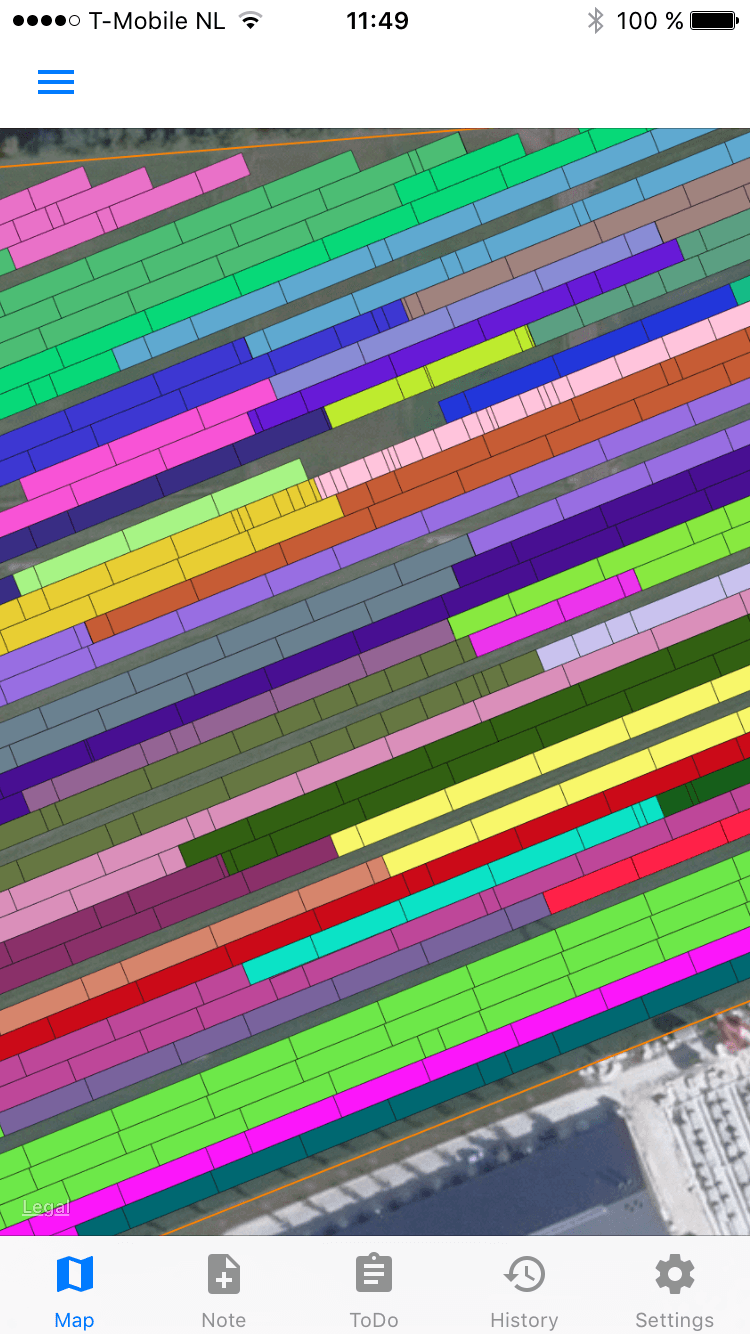
\includegraphics[width=0.5\textwidth,keepaspectratio=true]{BlockOverlay.png}
		\caption{Block overlay of field Grotto\label{fig:BlockOverlay}}
\end{figure}

As you can see in figure~\ref{fig:BlockOverlay} a field consists of a lot individual blocks, the amount depends on the size of the field but is somewhere in the several hundreds. This created some serious performance issues for the map. The map gets really unresponsive and slow after adding so many \glspl{polygon} to it. To reduce the stress on the map on iOS we added our own \gls{polygon} implementation that could contain many single \glspl{polygon}. This reduced the work needed by the map enormously, since the polygons for one field are drawn in one single draw and not every \gls{polygon} on his own. This made the map usable again but also introduce a delay when the polygons need be shown by the map. But this is the only working workaround for the performance problems. Further performance improvements could only be achieved by moving the map drawing to a server and only getting pre rendered \gls{maptiles} to display from it.


\subsection{Creating and Displaying HeatMaps}

\begin{figure}[h]
		\centering
		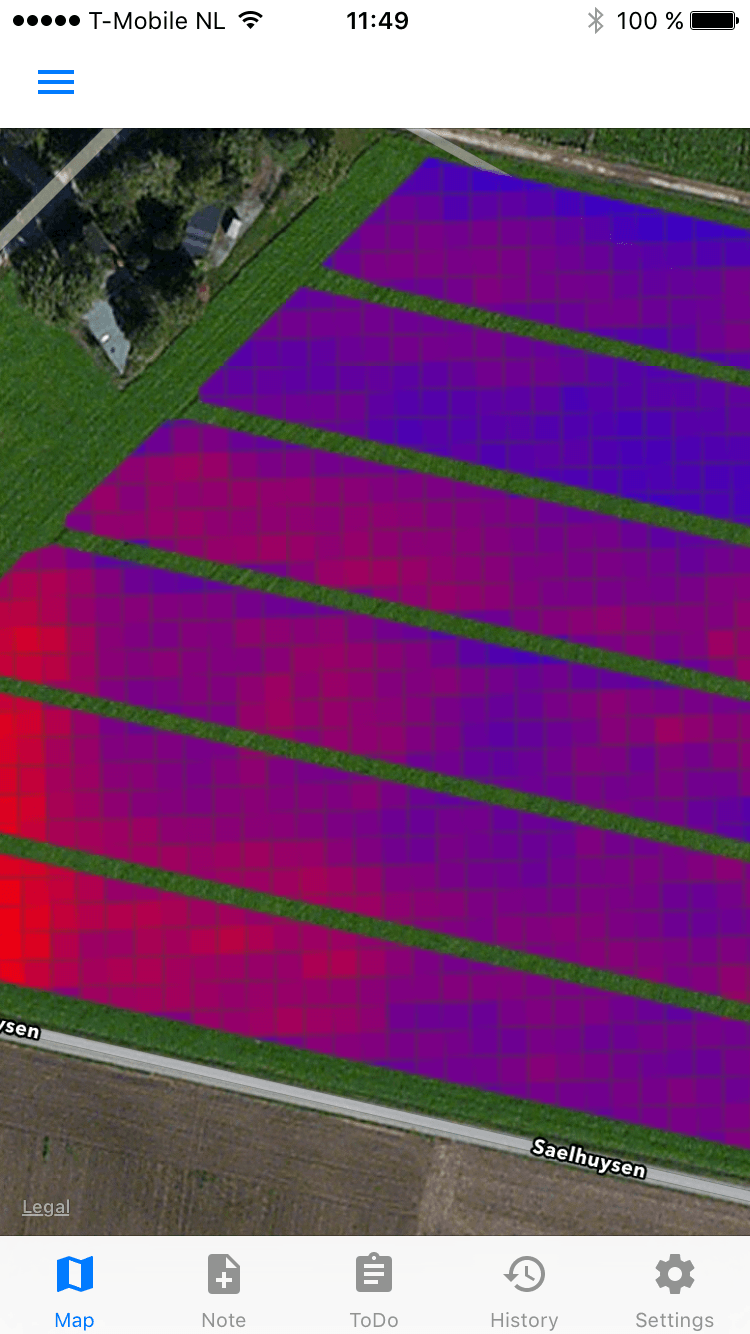
\includegraphics[width=0.5\textwidth,keepaspectratio=true]{HeatMap.png}
		\caption{Heatmap inside of the iOS \gls{app}\label{fig:Heatmap}}

\end{figure}

Another feature that was implemented for the map was the display of heat maps, these should show data like a soil scan that is not bound to specific blocks but more to specific points on the field.

The first try of implementing heat maps included displaying an image \glspl{overlay} created from the data and putting that on top of the map. For this approach we found a working Objective C Library called LFHeatMap \citet{LFHeatMaps}. To use it in our project we created a C\# Binding for it.
This was really easy to do following the tutorial on the Xamarin site \citet{bindingtut}. But this created heat maps based on single weighted points. Since we only got heat map data from Fleuren that contained of polygons with data, we looked for another solution.

As you can see in figure~\ref{fig:Heatmap} we implemented the heat map as just a bunch of polygons. The colors of the polygons were calculated based on their data. The color moves from solid blue for the lowest values to solid red for the highest values. The heat map displayed consists of about 4000 different polygons. The approach therefore is more a proof of concept since the drawing on the map takes several seconds and doesn't even work on android.

\subsection{Importing KML files into the app}
Fleuren supplied us with various datasets from their fields, to test our implementation with real data, especially the amount of data, we implemented a mechanism to read these files. The data we got was mostly shapefiles, since there is no easy way to read these we converted them to 
\gls{kml} files. \gls{kml} is basically just a version of \gls{xml} which is designed for geospatial data. To convert the files we used the .Net xml parsing library. 

\subsection{Geofencing}

The \gls{Geofencing} part of the application is based on the plugin which can be found at \url{https://github.com/domaven/xamarin-plugins/tree/master/Geofence}. This plugin has most of the functionality that is required in the project, however the plugin is outdated and does't work anymore. \\
To make the most out of Xamarin, most of the work should be done in the Forms application, this way code is reused for both Android and iOS. The class diagram on the next page shows what classes are in the Forms application. \\ 
The IGeofence and IGeofenceStore are interfaces that should be implemented in a platform specific way, because they contain the actual geofences and their platform specific way of working. The IGeofenceStore interface has some methods that can be shared between the platforms, therefor an abstract class BaseGeofenceStore is created, that has these methods already implemented.\\
The CrossGeofence class is responsible for creating the actual platform specific implementation of the IGeofence interface. This is done by using \href{https://developer.xamarin.com/guides/xamarin-forms/dependency-service/}{DependencyService} to get the actual platform specific implementation. \\
The platform specific code calls the methods in the CrossGeofenceListener class inside the Forms project, this way state changes can be handled in a universal way, instead of platform specific.

\newpage
\begin{figure}
	\begin{tikzpicture}
			\begin{class}[text width=4.5cm]{GeofenceCircularRegion}{10.2,-14}
				\attribute{Id : String}
				\attribute{Latitude : double}
				\attribute{Longtitude : double}
				\attribute{Radius : double}
				\attribute{NotifyOnEntry : bool}
				\attribute{NotifyOnStay : bool}
				\attribute{NotifyOnExit : bool}
			\end{class}

			\begin{class}[text width=4.5cm]{GeofenceLocation}{10.2, -10.2}
				\attribute{Latitude : double}
				\attribute{Longtitude : double}
				\attribute{Date : DateTime}
				\attribute{Accuracy : double}
			\end{class}

			\begin{interface}[text width=4.5cm]{IGeofence}{0,0}
				\attribute{Regions : IReadOnlyDictionary\textless string, GeofenceCircularRegion\textgreater}
				\attribute{GeofenceResults : IReadOnlyDictionary\textless string, GeofenceResult\textgreater}
				\attribute{IsMonitoring : bool}
				\attribute{LastKnownLocation : GeofenceLocation}
				\operation{StartMonitoring(region : GeofenceCircularRegion) : void}
				\operation{StartMonitoring(regions : IList \textless GeofenceCircularRegion\textgreater) : void}
				\operation{StopMonitoring(id : string) : void}
				\operation{StopMonitoring(ids : IList\textless string\textgreater) : void}
				\operation{StopMonitoringAll\-Regions() : void}
			\end{interface}

			\begin{class}[text width=4.5cm]{CrossGeofence}{0,-14}
				\attribute{Implementation : IGeofence}
				\attribute{GeofenceListener : IGeofenceListener}
				\attribute{IsInitialized : bool}
				\attribute{Current : IGeofence}

				\operation{Initialize(GeofencePriority geofencePrioriy, float smallesDisplacement) : void}
				\operation{CreateGeofence() : IGeofence}
			\end{class}

			\begin{interface}[text width=4.5cm]{IGeofenceStore}{10.2,0}
				\operation{GetAll() : Dictionary\textless string, GeofenceCircularRegion\textgreater}
				\operation{Get(string id) : GeofenceCircularRegion}
				\operation{Save(GeofenceCircular\-Region region) : void}
				\operation{RemoveAll() : void}
				\operation{Remove(string id) : void}
			\end{interface}

			\begin{abstractclass}[text width=4.5cm]{BaseGeofenceStore}{10.2,-6.7}
				\implement{IGeofenceStore}
				\operation{\#GetFieldKey(string id, string fieldName) : string}
			\end{abstractclass}
			
			\begin{interface}[text width=4.5cm]{IGeofenceListener}{5.1,0}
				\operation{OnMonitoringStarted(id : string) : void}
				\operation{OnMonitoringStopped() : void}
				\operation{OnMonitoringStopped(id : string) : void}
				\operation{OnRegionStateChanged( result : GeofenceResult) : void}
				\operation{OnError(error: string) : void}
			\end{interface}

			\begin{class}[text width=4.5cm]{CrossGeofenceListener}{5.1,-14}
				\operation{OnMonitoringStarted(\-string region) : void}
				\operation{OnMonitoringStopped(\-string region) : void}
				\operation{OnMonitoringStopped() : void}
				\operation{OnError(string error) : void}
				\operation{OnRegionStateChanged( GeofenceResult result) : void}
			\end{class}
	\end{tikzpicture}
	\caption{Geofencing class diagram\label{fig:GeofenceClassDiagram}}
\end{figure}
